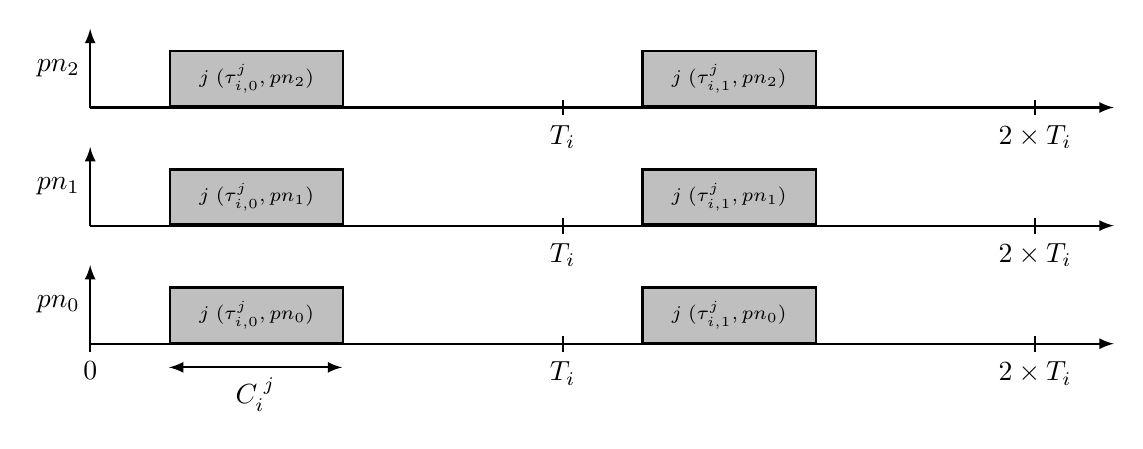
\begin{tikzpicture}
\draw[thick, -latex] (0,0) -- (13,0);
\draw[thick, -latex] (0,1.5) -- (13,1.5);
\draw[thick, -latex] (0,3) -- (13,3);
\draw[thick, -latex] (0,0) -- (0,1) node[midway, left] {$pn_0$};
\draw[thick, -latex] (0,1.5) -- (0,2.5) node[midway, left] {$pn_1$};
\draw[thick, -latex] (0,3) -- (0,4) node[midway, left] {$pn_2$};


\draw  (1,3) node[draw, thick, fill=lightgray, rectangle, anchor=south west, inner sep=0pt, minimum width=2.2cm, minimum height=0.7cm]      {\scriptsize $ j \; ( \tau_{i,0}^j, pn_2 )$};
\draw  (1, 1.5) node[draw, thick, fill=lightgray, rectangle, anchor=south west, inner sep=0pt, minimum width=2.2cm, minimum height=0.7cm]   {\scriptsize $ j \; ( \tau_{i,0}^j, pn_1 )$};
\draw  (1,0) node[draw, thick, fill=lightgray, rectangle, anchor=south west, inner sep=0pt, minimum width=2.2cm, minimum height=0.7cm]      {\scriptsize $ j \; ( \tau_{i,0}^j, pn_0 )$};
\draw[thick, latex-latex] (1,-0.3) -- (3.2,-0.3) node[midway, below] {$C_i^{\; j}$};

\draw[thick] (0,0.1) -- (0, -0.1) node [below] {$0$};
\draw[thick] (6,0.1) -- (6, -0.1) node [below] {$T_i$};
\draw[thick] (6,1.6) -- (6, 1.4) node [below] {$T_i$};
\draw[thick] (6,3.1) -- (6, 2.9) node [below] {$T_i$};


\draw[thick] (12,1.6) -- (12, 1.4) node [below] {$2 \times T_i$};
\draw[thick] (12,0.1) -- (12, -0.1) node [below] {$2 \times T_i$};
\draw[thick] (12,3.1) -- (12, 2.9) node [below] {$2 \times T_i$};

\draw  (7,0) node[draw, thick, fill=lightgray, rectangle, anchor=south west, inner sep=0pt, minimum width=2.2cm, minimum height=0.7cm]      {\scriptsize $ j \; ( \tau_{i,1}^j, pn_0 )$};
\draw  (7, 1.5) node[draw, thick, fill=lightgray, rectangle, anchor=south west, inner sep=0pt, minimum width=2.2cm, minimum height=0.7cm]   {\scriptsize $ j \; ( \tau_{i,1}^j, pn_1 )$};
\draw  (7,3) node[draw, thick, fill=lightgray, rectangle, anchor=south west, inner sep=0pt, minimum width=2.2cm, minimum height=0.7cm]      {\scriptsize $ j \; ( \tau_{i,1}^j, pn_2 )$};
\end{tikzpicture}
